\subsection{Motivation}

% TLP is a great tool for esd analysis
Throughout this document and in the \gls{esd} field in general, the \gls{tlp} generator is used extensively as a characterization and testing tool.
Amoung its many advantages, it generates very clean and controllable pulses in a shielded environment.
It has also proven to be a great tool for studying, among other things, the behavior of silicon-level devices.

% But ESD gun is required.
Nevertheless, \gls{esd-gun} testing remains the mandatory requirement defined by customers for product qualification.
\gls{tlp} testing alone is not a sufficient proof for customers that the integrated circuit can survive the harsh real environment, especially for automotive applications.
Several \gls{esd-gun} standards exist, targeting qualification of devices against electro-static discharges.
The HMM specification \cite{hmm}, the IEC 61000-4-2 standard \cite{iec61000-4-2} and the ISO 10605 standard \cite{iso10605} define the same \gls{esd} testing waveform, using the same discharge device, but with different application conditions.
Together, they cover a very large amount of tested devices from equipment, boards, and integrated circuit, in automotive and consumer fields.
The waveform common to those three standards (Fig. \ref{fig:hmm-waveform}) is virtually the most widely used pulse for ESD qualification.

\begin{figure}[!h]
  \centering
  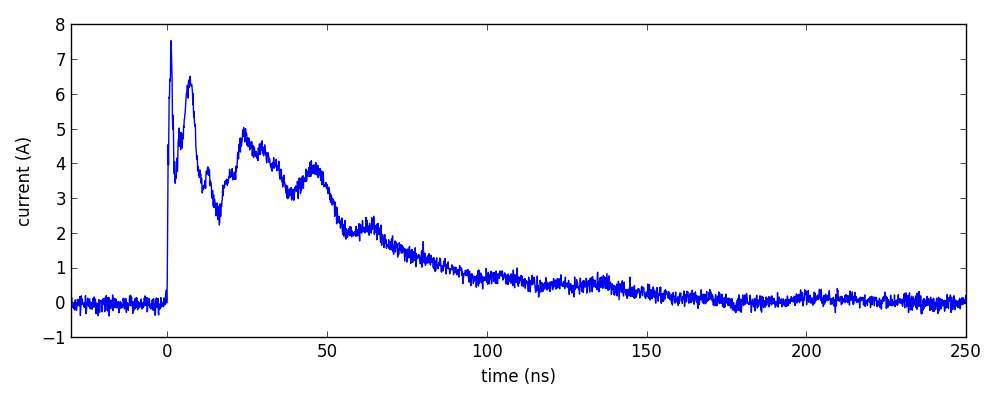
\includegraphics[width=0.3\textwidth]{src/5/figures/hmm_pulse.pdf}
  \caption{HMM pulse current waveform - 1kV charging voltage on a 2\textOmega{} load}
  \label{fig:hmm-waveform}
\end{figure}

% Main problems with Gun
By design, the \gls{esd-gun} has certain requirements to generate a realistic \gls{esd} discharge.
Incidentally, those requirements make investigation harder because the injected waveform and test conditions are less reproducible \cite{hmm-round-robin-study}.
For instance, injection is performed through a metallic tip a few centimeters long.
The tip is a large source of electomagnetic radiated noise during the discharge up to several gigahertz \cite{system-level-esd-failure-variation}.
Also, the ground return is a metallic ribbon a few meters long.
It models the equivalent ground connection of a human body.
However, it is also very inductive, and its value changes considerably in function of its shape.
Finally, for integrated circuits in particular, the ESD gun waveform is a lot more complex than the rectangular TLP shape.
In case of failure, the investigation can be quite tedious to conduct.

% Correlation between TLP and Gun
Unlike the ESD gun, \gls{tlp} generators are extremely well controlled.
The discharge propagates entirely inside coaxial cables and does not generate any \gls{rf} radiation.
In some few cases, failures can be correlated between a \gls{tlp} and \gls{esd-gun} \cite{correlation-system-level-esd-tlp}.
However, there is generally no clear link between failures induced by each generator \cite{miscorrelation-esd-hmm}.
The lack of correlation is proven further in \cite{correlation-system-level-esd-tlp}, with 2k\textOmega{} ESD gun discharge modules.
\cite{correlation-system-level-esd-tlp} demonstrates that some ESD structures in analog high-voltage technology have completely uncorrelated failure levels between TLP and HMM. Failure analysis shows that the failure mechanisms are different.

% Motivation
Therefore, \gls{tlp} cannot be used as a drop-in replacement to \gls{esd} gun for qualification.
A compromise can be found by modifying a \gls{tlp} generator to produce the gun waveform, but in a shielded, well-controlled, and reproducible environment.
This approach has been explored in the past by E. Grund \cite{iec61000-tlp} and Y. Cao \cite{tlp-based-hmm}.

% Explain Grund setup
In \cite{iec61000-tlp}, Grund modifies a TLP generator by placing an impedance mismatch between two coaxial lines.
The architecture of the device is given in Fig. \ref{fig:grund_tlp_hmm}.
With this setup, the initial peak of the waveform is produced by a 4ns cable.
The second part of the waveform is produced by the combination of the 30ns cable and a large series resistance R\textsubscript{ML}, that lowers the current compared to the first peak.
A risetime filter connected after the switch enforces a maximum risetime of 700ps to 1ns, to match the value defined in the standards.
Overall, the generated waveforms has less dynamic than the standardized waveform and exhibits two flat steps.
It is also widely unmatched because of the series resistor.
It is suspected that this impedance mismatch placed between two delays makes this generator very likely to generate oscillations.
The mismatch causes travelling waves to bounce back and forth between the load and R\textsubscript{ML}, and this kind of behavior is quite far from an original gun generator.
It does comply to the standards though since the required values for risetime, current at 30ns and 60ns are comprised in the tolerance margins.

\begin{figure}[!h]
  \centering
  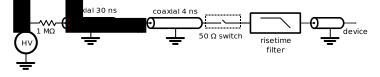
\includegraphics[width=0.9\textwidth]{src/5/figures/grund_tlp_hmm.pdf}
  \caption{Grund's modified TLP for HMM pulse generation}
  \label{fig:grund_tlp_hmm}
\end{figure}

% Explain Cao setup
The approach proposed by Cao in \cite{tlp-based-hmm} consists in employing a capacitive discharge through a short coaxial cable to generate an HMM-compliant pulse.
The architecture of the device is given in Fig. \ref{fig:cao_tlp_hmm}.
The generator cannot be really classified as a \gls{tlp} generator, since the discharge is mostly supported by the RLC network. The 1ns coaxial cable acts as a distributed capacitor to provide the high current of the first peak.
Overall, the generated waveform look good on a 50\textOmega{} load.
However, the system is always verified with a 50\textOmegae{} termination.
It is never tested in mismatched output conditions, with a true pure 2\textOmega{} resistive load as defined in the standard.
It is suspected that with an impedance mismatch at the output, the system enters in ringing oscillation.
The oscillation is likely generated by an energy exchange between the load and the RLC network, separated by the delay of the injection cable.
Ultimately, this generator is probably not compliant with the standard.

\begin{figure}[!h]
  \centering
  
\includegraphics[width=0.9\textwidth]{src/5/figures/cao_tlp_hmm.pdf}
  \caption{Cao's TLP-based HMM generator}
  \label{fig:cao_tlp_hmm}
\end{figure}

% What is proposed here is a different architecture for tlp-hmm generator
In this chapter, a new and different setup is proposed.
It is based on using propation delays to shape the pulse with high flexibility.
Compared to those two previous approaches, the design proposed in this document works with a classic 100 ns \gls{tlp}, without requiring internal modifications.
It will be demonstrated later that the proposed architecture is quite flexible, and can be tuned to match any gun pulse configuration.
It is also possible to tune the output impedance, while still keeping the same waveform.
Ultimately, this generator is able to generate an HMM waveform inside a shielded environment, but with a large output impedance similarly to true HMM generators.
This generator was published in \cite{my-publi-tlp-hmm}.
